\newtcolorbox{textBox}[1][]{
 parbox=false,
 			colback=Teal!10,
 			colframe=Teal,
 			colbacktitle=Teal,
 			enhanced jigsaw,
 			breakable,  
 			attach boxed title to top text left={yshift=-3mm,yshifttext=-3mm}, 
 			#1,%
}

\chapter{Einführung in die Globalisierung und globale Lieferketten}
\begin{myexercise}
Untersuchen Sie die Etiketten Ihrer Kleidungsstücke und beantworten Sie folgende Fragen:
\begin{itemize}
\item In welchem Land wurde das Kleidungsstück hergestellt?
\item Wo haben Sie das Kleidungsstück gekauft?
\item Welche Materialien sind laut Etikett enthalten?
\end{itemize}
\notiz{6}

\begin{myanswer}
Mögliche Lösung:
\begin{enumerate}
\item Hergestellt in:
\begin{itemize}
\item Bangladesch, China, Türkei, Vietnam, Indien oder Pakistan
\item Manche hochwertige Produkte: Portugal, Italien, Deutschland
\end{itemize}

\item Gekauft in:
\begin{itemize}
\item Lokale Geschäfte, grosse Modeketten (H\&M, Zara, Uniqlo, Levi’s) oder Online-Shops
Materialien laut Etikett:
\item Baumwolle (z. B. aus den USA, Indien, China)
\item Polyester (synthetische Fasern, meist aus Erdölprodukten)
\item Elasthan (für Dehnbarkeit, oft in Sportkleidung enthalten)
\item Viskose (aus Zellulose, halbsynthetisch)
\end{itemize}

\end{enumerate}
\end{myanswer}
\end{myexercise}

\begin{myexercise}[Hypothesenbildung: Warum sind Lieferketten global?]\label{ex:globaleLieferketten}

Notieren Sie erste Hypothesen im Textfeld untenan und vervollständigen Sie danach folgendes Padlet: 

\qrcode{https://padlet.com/serafinschneider/ursachen-globalisierung-n4umvx8vos79ow8i}

\notiz{7}

\begin{myanswer}
\begin{itemize}
\item \textbf{Kostenvorteile}: Produktion in Ländern mit niedrigeren Lohnkosten reduziert die Herstellungskosten.
\item \textbf{Spezialisierung}: Unterschiedliche Länder sind auf bestimmte Produktionsschritte spezialisiert (z. B. Baumwollanbau in den USA, Textilproduktion in Bangladesch).
\item \textbf{Ressourcenverfügbarkeit}: Rohstoffe wie Baumwolle oder synthetische Fasern werden nicht überall angebaut oder produziert.
\item \textbf{Freihandel \& wirtschaftliche Anreize}: Internationale Handelsabkommen und geringe Zölle erleichtern die globale Produktion.
\item \textbf{Logistik \& Infrastruktur}: Verbesserte Transportmöglichkeiten (Containerschiffe, Flugfracht) ermöglichen weltweite Lieferketten.
\item \textbf{Marktnähe}: Grosse Modeketten produzieren in mehreren Ländern, um unterschiedliche Märkte schnell zu beliefern.
\end{itemize}
\end{myanswer}

\end{myexercise}

\begin{myexercise}[Die Reise einer Jeans]
Bevor eine Jeans in den Regalen der Handelskette landet, durchlebt sie eine sehr lange Reise. Hier sehen Sie exemplarisch aufgeführte Stationen, die eine Jeans von ihrem Ursprung bis zu ihrer finalen Destination durchläuft: Stellen Sie in der folgenden Karte die exemplarisch aufgeführten Arbeitsschritte dar:

\begin{itemize}
\item In Kasachstan oder Indien wird die Baumwolle geerntet.
\item In der Türkei wird die Baumwolle zu Garn gesponnen.
\item In Taiwan wird das Baumwollgarn mit chemischer lndigofärbe gefärbt. 
\item Aus dem Garn werden in Polen die Jeansstoffe gewebt.
\item Innenfutter und die kleinen Schildchen mit der Waschanleitung kommen aus Frankreich;Knöpfe und Nieten aus Italien.
\item Danach werden alle Einzelteile auf den Philippinen zusammengenäht.
\item In Griechenland erfolgt die Endverarbeitung mit Bimsstein.
\item Die Jeans werden in Österreich verkauft, getragen und schliesslich in die Altkleidersammlung einer karitativen Einrichtung gegeben.
\item In einem Betrieb in den Niederlanden wird die Kleidung dann sortiert.
\item Mit Schiffen und LKWs werden sie auf den afrikanischen Kontinent gebracht.
\end{itemize}

\begin{figure}[H]
\centering
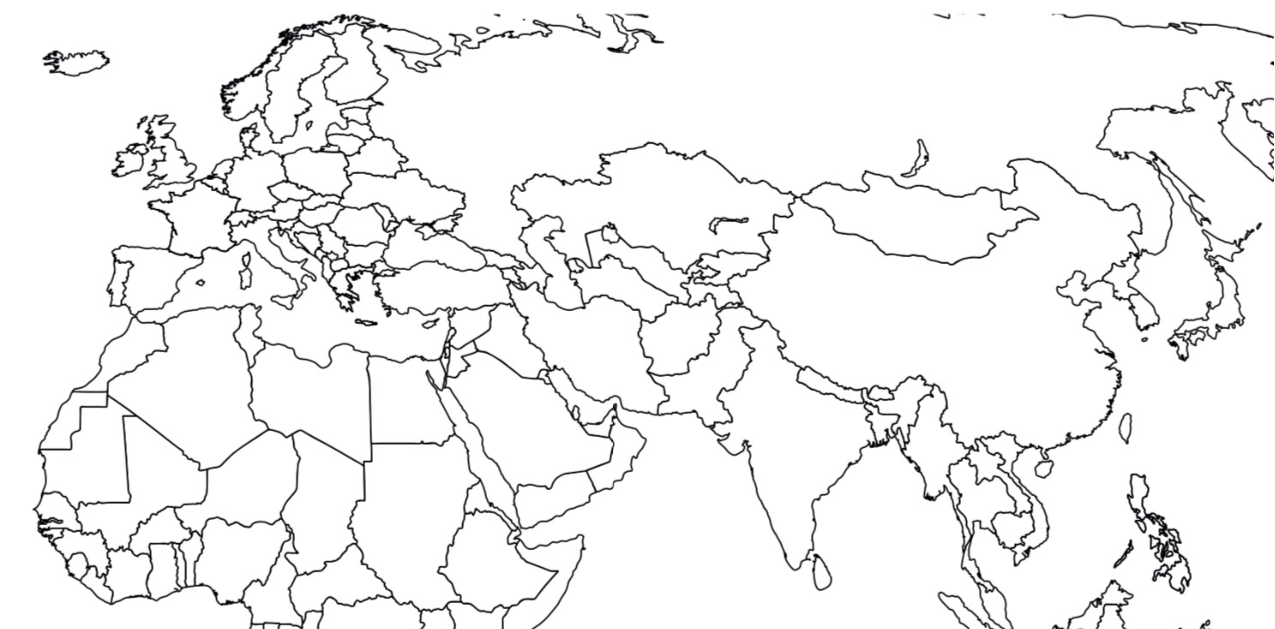
\includegraphics[width=\linewidth]{Geografie/LOFS/map-empty}
\caption{Leere Weltkarte für Jeans-Wertschöpfungskette \cite{umweltBildung}}
\end{figure}
\begin{myanswer}
\begin{figure}[H]
\centering
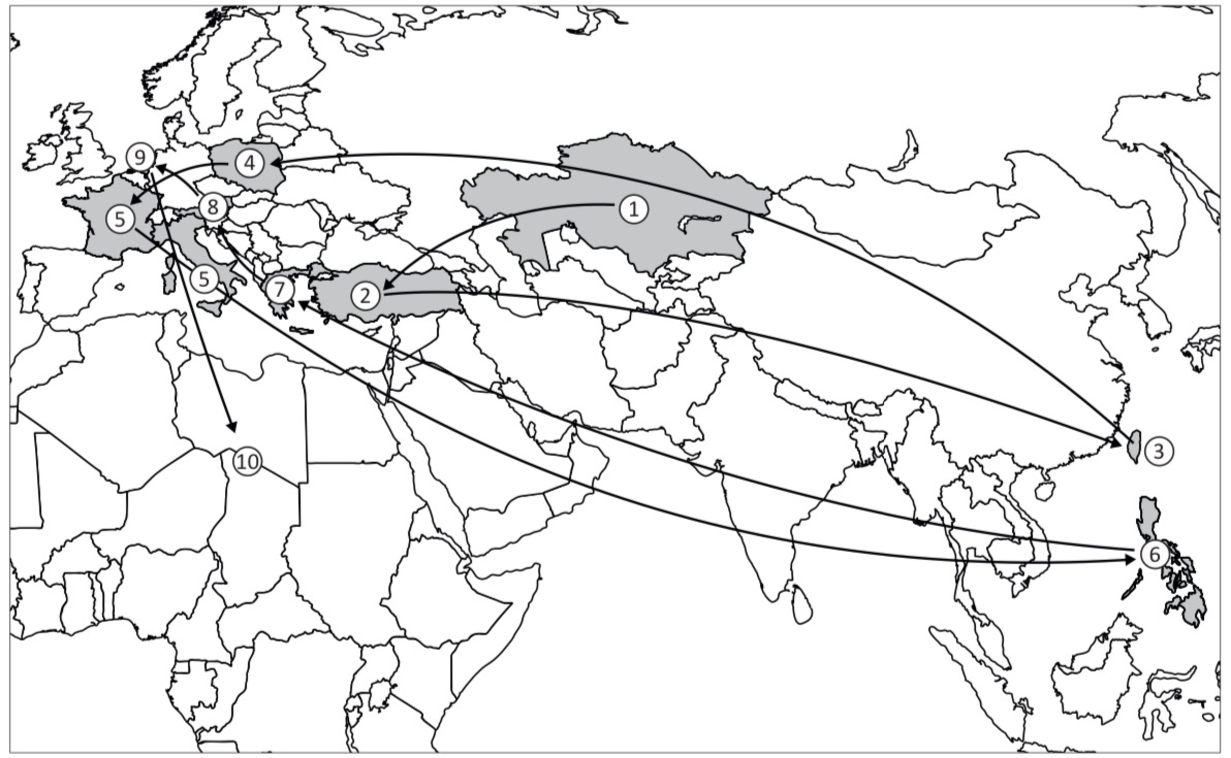
\includegraphics[width=\linewidth]{Geografie/LOFS/map-sol}
\caption{Weltkarte für Jeans-Wertschöpfungskette \cite{umweltBildung}}
\end{figure}

\end{myanswer}
\end{myexercise}

\begin{mychallenge}[Verkaufspreis einer Jeans]
\begin{enumerate}
\item Überlegen Sie sich, wie sich der Verkaufspreis einer Jeans zusammensetzt und ordnen Sie die prozentuale Verteilung des Preises den einzelnen Akteuren (Hersteller, Marke, Einzelhandel, Transport, etc.) auf \cref{fig:jeans-leer} zu.
\item Diskutieren Sie in Ihrer Gruppe: Ist die Verteilung fair? Welche Akteure profitieren am meisten?
\end{enumerate}
\begin{figure}[H]
\centering
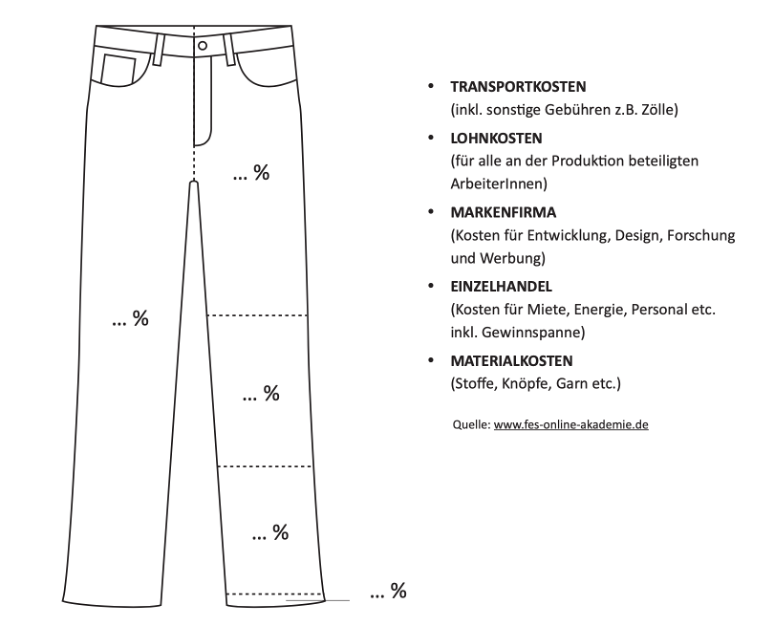
\includegraphics[width=.8\linewidth]{Geografie/LOFS/jeans-leer}
\caption{Jeans: Prozentualer Verkaufspreis \cite{umweltBildung}}
\label{fig:jeans-leer}
\end{figure}
\begin{myanswer}
\begin{figure}[H]
\centering
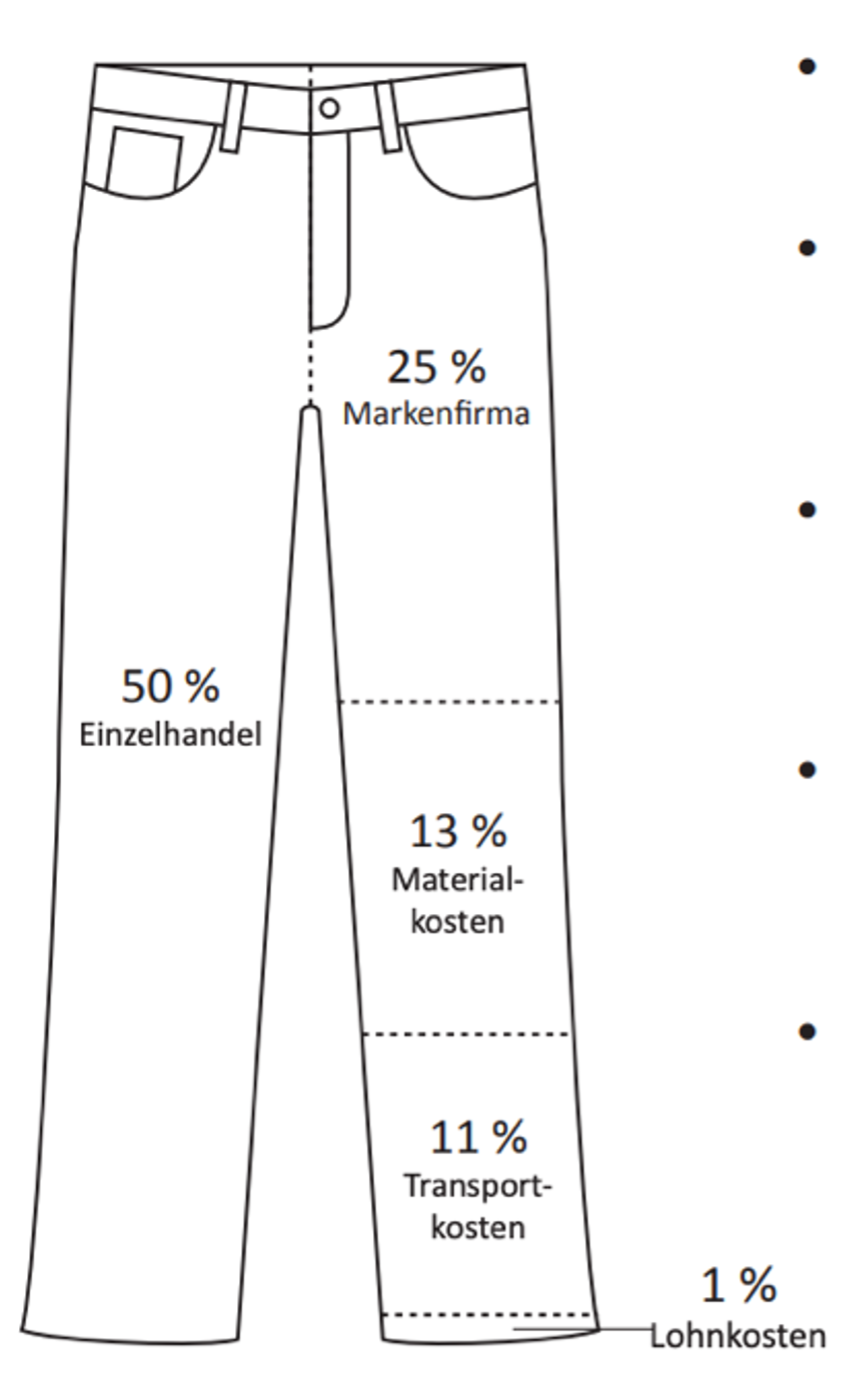
\includegraphics[width=.4\linewidth]{Geografie/LOFS/jeans-sol}
\caption{Jeans: Prozentualer Verkaufspreis (Musterlösung) \cite{umweltBildung}}
\end{figure}
\end{myanswer}

\end{mychallenge}

\begin{mydefinition}[Globalisierung]
\textbf{Globalisierung} ist die zunehmende weltweite Vernetzung in Wirtschaft, Politik, Kultur und Kommunikation. Sie ermöglicht den schnellen Austausch von Gütern, Informationen und Kapital über nationale Grenzen hinweg und führt zu einer stärkeren Interdependenz von Staaten, Unternehmen und Individuen.

\textbf{Geographisches Verständnis der Globalisierung:} In der Geografie beschreibt Globalisierung die räumliche Verflechtung wirtschaftlicher, politischer und gesellschaftlicher Prozesse über nationale Grenzen hinweg. Sie beeinflusst Lieferketten, Migration, Stadtentwicklung und Umwelt und führt zu regionalen Disparitäten, die Gewinner:innen und Verlierer:innen der Globalisierung hervorbringen.

\begin{figure}[H]
\centering
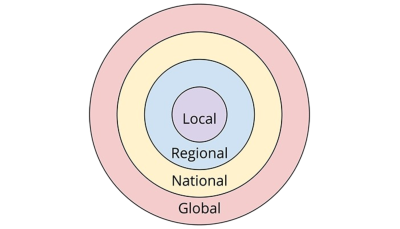
\includegraphics[width=.5\linewidth]{Geografie/LOFS/scales}
\caption{Skalen der Globalisierung}
\label{fig:scales}
\end{figure}
\notiz{5}
\end{mydefinition}
\clearpage

\begin{myexercise}
Ergänzen Sie das Padlet aus \cref{ex:globaleLieferketten} (\href{https://padlet.com/serafinschneider/ursachen-globalisierung-n4umvx8vos79ow8i}{Link}) mit ihren neuen Hypothesen, nachdem sie im Buch \enquote{Geografie - Wissen und Verstehen} \cite{hep} das Kapitel 14.6 \enquote{Entstehung der Globalisierung} gelesen haben.
\begin{myanswer}
Weitere Aspekte:

\begin{itemize}
\item \textbf{Kolonialismus als historische Grundlage}: Europäische Kolonialmächte etablierten Handelsrouten und Wirtschaftsstrukturen, die den globalen Austausch von Rohstoffen und Produkten förderten.
\item \textbf{Industrielle Revolution als Beschleuniger}: Technologische Fortschritte in der Produktion und im Transport (Dampfschiffe, Eisenbahn) ermöglichten den weltweiten Handel und Massenproduktion.
\item \textbf{Technologische Innovationen}: Digitalisierung, das Internet und moderne Logistiksysteme (z. B. Containerschifffahrt) haben Handelsprozesse vereinfacht und global vernetzt.
\item \textbf{Wachsender globaler Konsum}: Steigender Wohlstand in vielen Regionen führte zu einer höheren Nachfrage nach importierten Produkten und beschleunigte die globale Produktion.
\item \textbf{Liberalisierung der Märkte}: Abbau von Handelshemmnissen (Zölle, Importbeschränkungen) durch internationale Organisationen wie \gls{WTO}, \gls{IWF} und Weltbank förderte den weltweiten Handel.
\item \textbf{Ausbau internationaler Finanzmärkte}: Kapital kann heute grenzenlos investiert werden, wodurch Unternehmen Standorte dort aufbauen, wo Kosten und Bedingungen am besten sind.
\item \textbf{Globale Arbeitsteilung \& Spezialisierung}: Unternehmen verteilen Produktionsprozesse weltweit, um Lohn- und Ressourcenunterschiede effizient zu nutzen (z. B. Entwicklung in den USA, Produktion in China).
\item \textbf{Multinationale Unternehmen als Treiber}: Grosskonzerne bauen globale Produktionsnetzwerke auf und investieren in verschiedene Länder, um Märkte zu erschliessen.
\item \textbf{Politische Stabilität \& Global Governance}:
Internationale Organisationen (\gls{UN}, \gls{WTO}, \gls{EU}) und Handelsabkommen schaffen ein Umfeld, in dem globaler Handel sicherer und stabiler möglich ist.
\end{itemize}

\end{myanswer}
\end{myexercise}

\begin{myexercise}
\begin{enumerate}
\item Bilden Sie vier Gruppen (zu je 3 - 5 Personen) und wählen Sie eines der folgenden Produkte aus:
\begin{itemize}
\item Schokolade
\item Fleisch
\item Kleidung
\item Smartphone
\end{itemize}

\item Erstellen Sie auf einem Flipchart eine umfassende Lieferkette für Ihr Produkt. Material (Dossiers, Links, etc.) für ihre Recherche finden Sie im Ordner \enquote{Unterrichtsmaterial auf Teams} unter dem von Ihnen gewähltem Produkt. Berücksichtigen Sie folgende Aspekte:
\begin{enumerate}
\item Welche \textbf{Akteure} spielen eine Rolle? 
\item Welche \textbf{Länder} sind beteiligt? 
\item Welche \textbf{wirtschaftlichen, sozialen und ökologischen} Aspekte sind relevant?
\item Spezialfall herausarbeiten: Gibt es besondere Akteure, die nur für Ihr Produkt relevant sind, oder für ihr Produkt essentiell sind?
\end{enumerate}
\item Färben Sie mögliche Auswirkungen oder Prägungen einzelner Akteure mit den Farben des Skalen-Konzept (s. \cref{fig:scales}) ein. 
\end{enumerate} 
\begin{myanswer}
Keine Musterlösung, da unterschiedliche Antworten pro Gruppe möglich.
\end{myanswer}

\end{myexercise}
\chapter{Akteure der Globalisierung}

\begin{myexercise}
Während des Lehrvortrags zu den exogenen und endogenen Ursachen wirtschaftlicher Entwicklung machen Sie sich Notizen zu den wichtigsten Punkten. Achten Sie darauf, Beispiele und zentrale Begriffe festzuhalten.

Notieren Sie \textbf{zwei konkrete Beispiele für endogene Ursachen} sowie \textbf{zwei konkrete Beispiele für exogene Ursachen}:

\notiz{7}

\end{myexercise}

\begin{myexercise}[Fragmentierte Entwicklung]\label{ex:frag}
Lesen Sie den Text zur fragmentierten Entwicklung und bearbeiten Sie folgende Aufgaben:
\begin{enumerate}
\item Welche drei Raumtypen unterscheidet Scholz im Modell der fragmentierten Globalisierung?
\item Warum profitieren nicht alle Regionen und Gesellschaftsschichten gleichermassen von der Globalisierung?
\end{enumerate}

\begin{figure}[H]
\centering
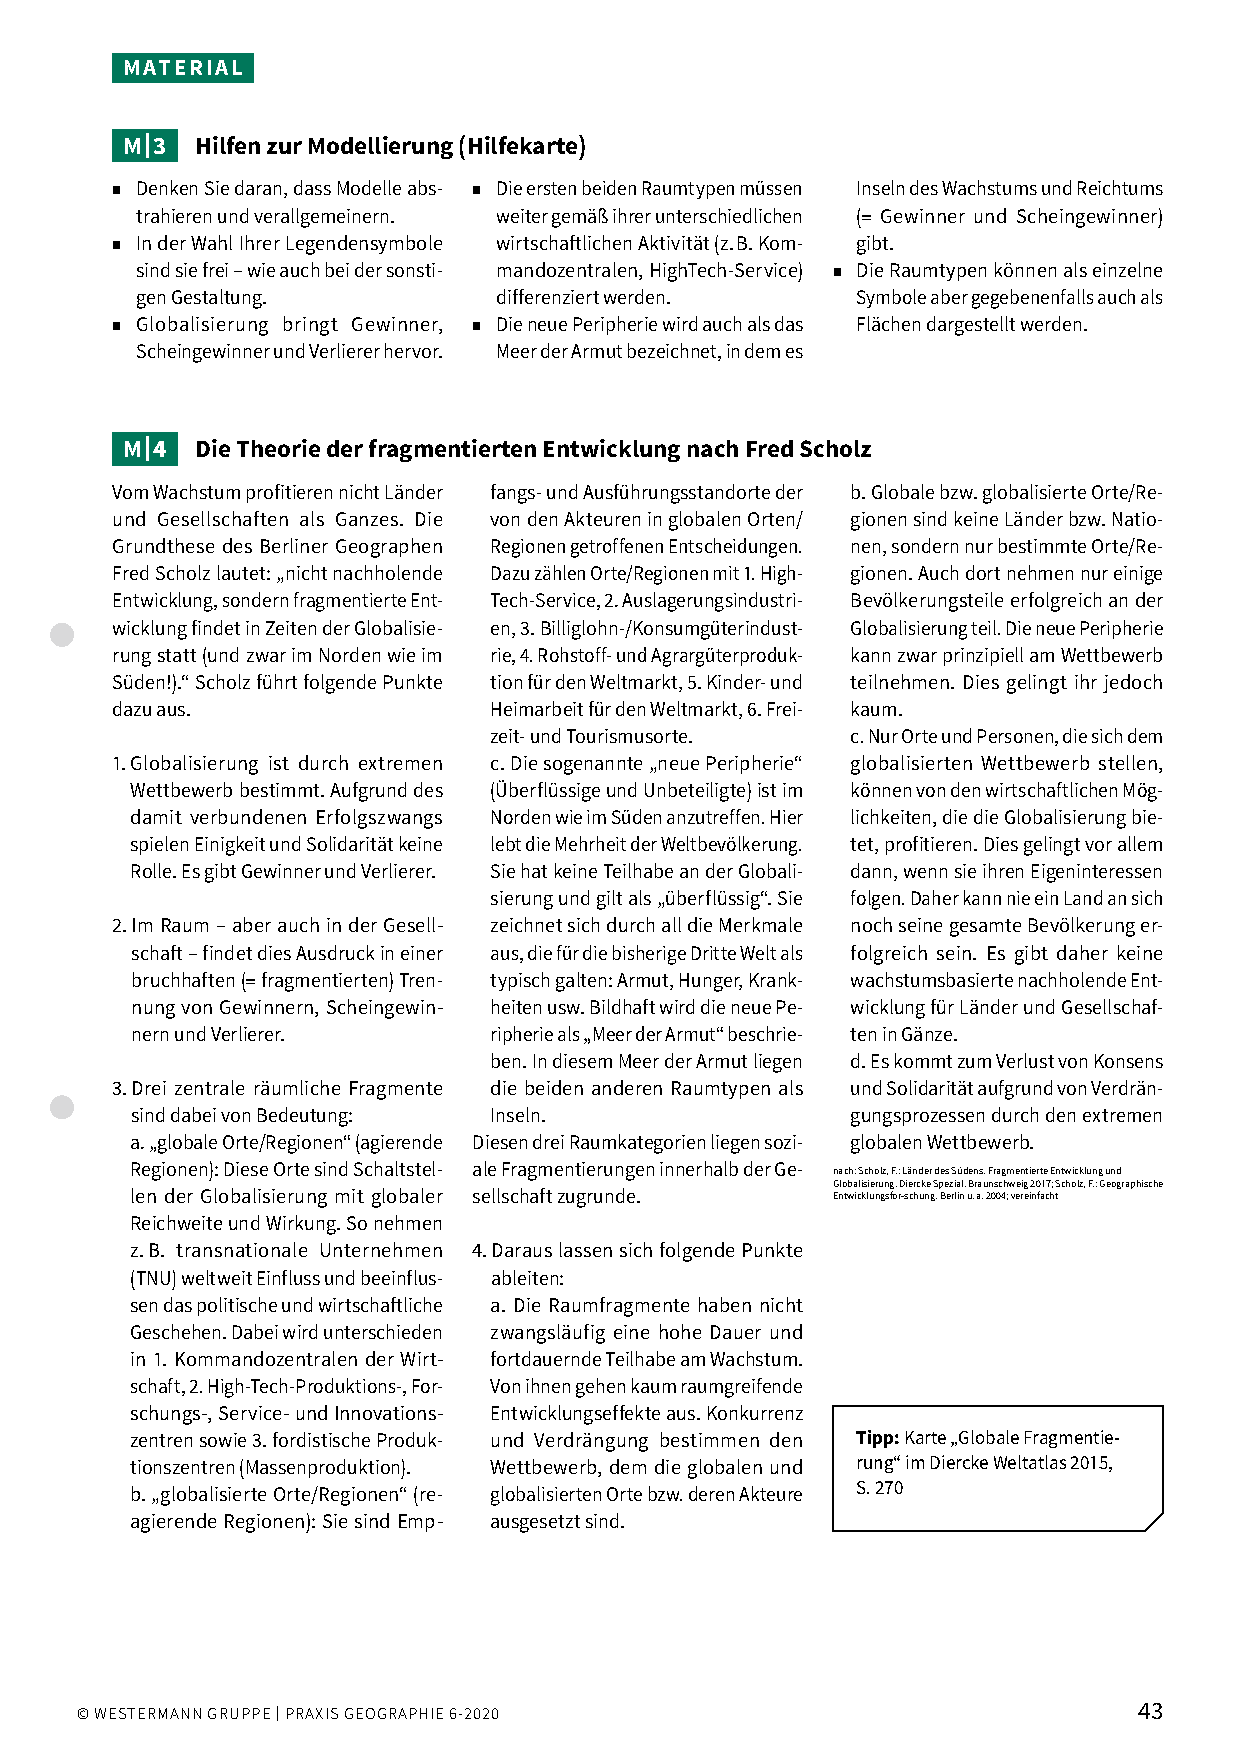
\includegraphics[trim={1cm 3cm 1cm 7cm},clip,width=\linewidth]{Geografie/LOFS/Fragmentierte}
\caption{Text zur Fragmentierten Entwicklung aus \cite{alma99117114725005511}}
\label{fig:fragmentierte}
\end{figure}
\end{myexercise}

\begin{myexercise}
Ergänzen Sie Abbildung \cref{fig:frag} mit typischen Akteuren aus dem Text aus \cref{ex:frag}.
\begin{figure}[H]
\centering
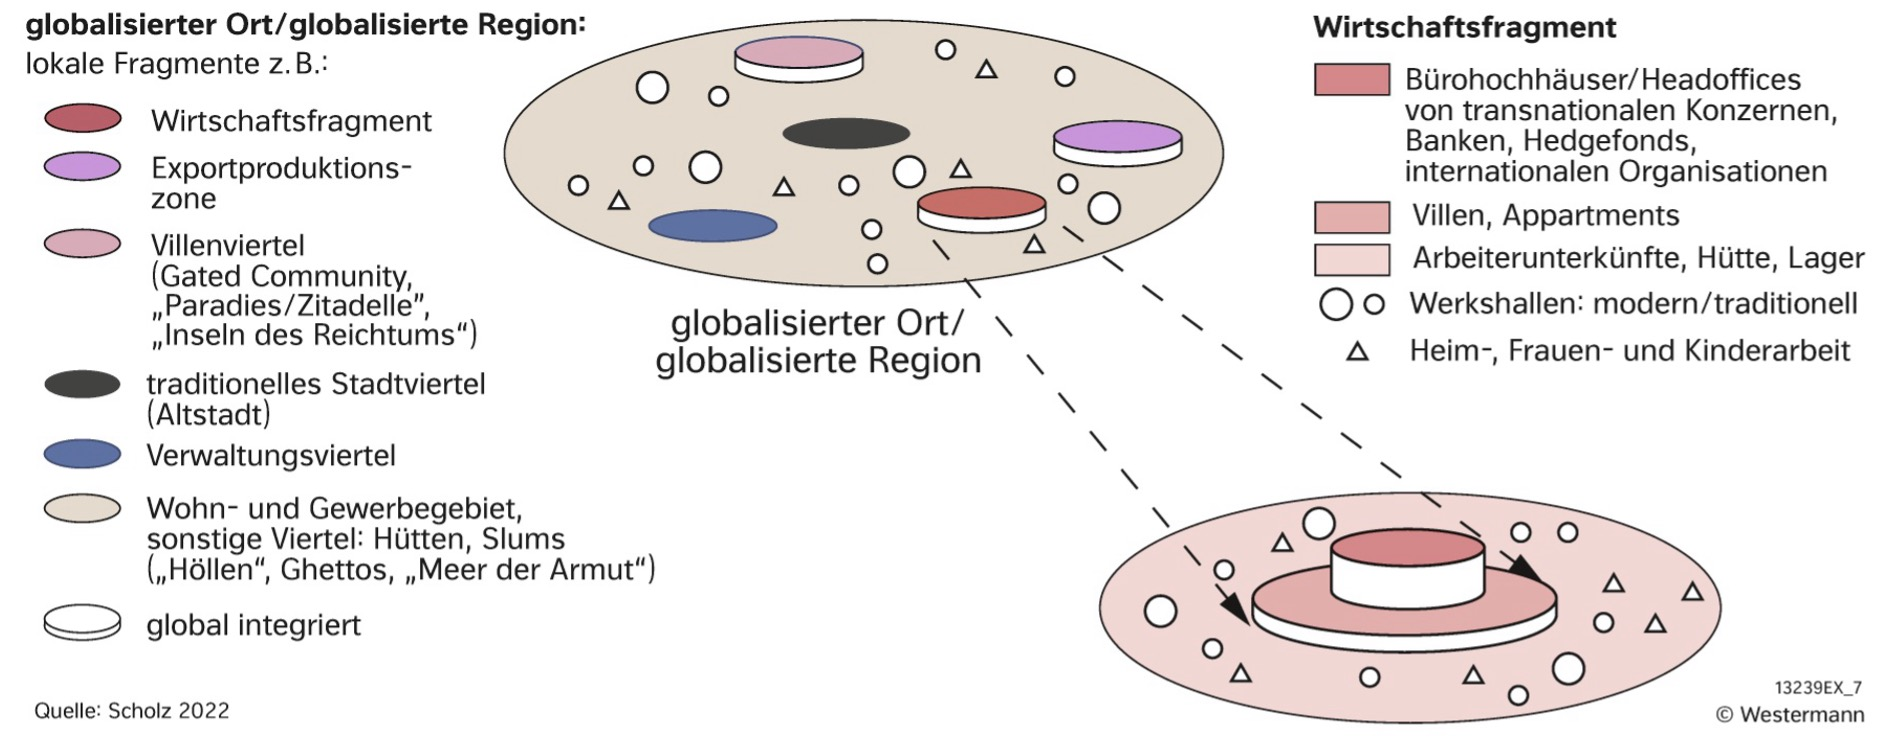
\includegraphics[width=.6\linewidth]{Geografie/LOFS/frag}
\caption{Fragmentierungs-Modell \cite{westermann}}
\label{fig:frag}
\end{figure}
\end{myexercise}

\begin{myexercise}[Global Cities und Global Players analysieren]
Schauen Sie sich das folgende Video an: 

\qrcode{https://www.youtube.com/watch?v=wg9eUGBiOH8&ab_channel=Geographie-simpleclub}

Beantworten Sie folgende Fragen dazu:
\begin{enumerate}
\item Was unterscheidet Global Cities von anderen Städten, und warum sind sie wirtschaftlich besonders wichtig?
\item Welche Rolle spielen Global Players in internationalen Produktions- und Handelsnetzwerken?
\end{enumerate}
\notiz{6}
\begin{myanswer} 
\textbf{1. Global Cities:}
\begin{itemize} 
\item Zentrale Rolle in der Weltwirtschaft
\item Sehr gute Verkehrs- und Kommunikationsinfrastruktur
\item Sitz internationaler Dienstleistungsunternehmen
\item Politisch und wirtschaftlich stark vernetzt
\item Steuerungs- und Kontrollzentren globaler Aktivitäten
\end{itemize}

\textbf{2. Global Players:}
\begin{itemize} \item Multinationale Unternehmen mit weltweiten Tochterfirmen
\item Grosse finanzielle und technische Ressourcen
\item Ziel: günstige Produktion, weltweiter Absatz
\item Einfluss auf Politik durch wirtschaftliche Macht
\item Beispiele: Walmart, Autohersteller
\end{itemize} 
\end{myanswer}
\end{myexercise}

\begin{myexercise}[ADI]
Schauen Sie sich das folgende Video an: 
\href{https://www.youtube.com/watch?v=xkAhublCT9g&t=18s&ab_channel=Geographie-simpleclub}{Link}

\textbf{Teil 1}: Notieren Sie sich die wichtigsten Begriffe in eigenen Worten:

\begin{itemize}
\item \gls{ADI}
\item Greenfield-Investitionen
\item Brownfield-Investitionn
\item \gls{MNU}
\item Standortwahl \& Standortfaktoren
\end{itemize}
\notiz{8}
\textbf{Teil 2}: Speed-Dating – Austausch 

\begin{itemize}
\item Finden Sie eine Person die gleich weit ist wie Sie.
\item Erklären Sie sich gegenseitig, welche Erkenntnisse Sie aus den Videos und dem Modell der fragmentierten Globalisierung gewonnen haben.
\end{itemize}
Platz für Notizen \& Erkenntnisse aus dem Austausch:
\notiz{8}

\begin{myanswer}
\begin{itemize}
  \item \textbf{\gls{ADI}:}  
  Investition eines Akteurs in ein Unternehmen oder Projekt im Ausland, z.B. durch Kapital, Wissen oder Technologie, um Vorteile oder Einfluss zu gewinnen.

  \item \textbf{Greenfield-Investitionen:}  
  Aufbau eines neuen Standorts im Ausland auf ungenutztem Land, inklusive neuer Gebäude und Infrastruktur.

  \item \textbf{Brownfield-Investitionen:}  
  Nutzung oder Umbau bestehender Anlagen im Ausland zur schnellen und kostengünstigen Aufnahme der Produktion.

  \item \textbf{\gls{MNU}:}  
  Unternehmen mit Standorten in mehreren Ländern, die global produzieren und investieren.

  \item \textbf{Standortwahl \& Standortfaktoren:}  
  Kriterien wie niedrige Löhne, geringe Umweltauflagen, Steuervergünstigungen oder gute Infrastruktur beeinflussen die Wahl des Investitionsstandorts.
\end{itemize}
\end{myanswer}

\end{myexercise}

\begin{myexercise}[Kategorisierung von Akteuren in der Jeans-Produktion]
Füllen Sie die folgende Tabelle aus. Identifizieren Sie zentrale Akteure in der Jeans-Lieferkette (z. B. Baumwollproduzenten, Hersteller, Marken, Einzelhandel) und ordnen Sie sie in die 3 Kategorien nach Scholz (Globale Orte, Globalisierte Orte, Neue Peripherie) ein.

\begin{table}[H]
\centering
\small
\begin{tabular}{p{4cm}||p{6cm}|p{4cm}}
\textbf{Akteur} & \textbf{Funktion in der Lieferkette} & \textbf{Kategorie nach Scholz }\\
\midrule\midrule
Baumwollplantagen & & \\[1.5cm]\midrule
Textilfabriken & & \\[1.5cm]\midrule
Modekonzerne (z. B. Levi’s, H\&M) & & \\[1.5cm]\midrule
Einzelhandel & & \\[1.5cm]\midrule
Logistikunternehmen & & \\[1.5cm]\midrule
Finanzdienstleister \& Banken & & \\[1.5cm]\midrule
Konsument:innen & & \\[1.5cm]\midrule
NGOs \& Arbeitsrechtsorganisationen & & \\[1.5cm]
\end{tabular}
\end{table}
\begin{myanswer}
\begin{table}[H]
\small
\centering
\begin{tabular}{p{4cm}||p{5cm}|p{3cm}}
\textbf{Akteur} & \textbf{Funktion in der Lieferkette} & \textbf{Kategorie nach Scholz }\\
\midrule\midrule
Baumwollplantagen & Rohstoffproduktion & Peripherie \\\midrule
Textilfabriken & Herstellung von Jeans & Globalisiert \\\midrule
Modekonzerne (z. B. Levi’s, H\&M) & Vertrieb \& Marketing & Global \\\midrule
Einzelhandel & Verkauf der Produkte & Globalisiert \\\midrule
Logistikunternehmen & Transport \& Verteilung & Globalisiert \\\midrule
Finanzdienstleister \& Banken & Investitionen \& Kreditvergabe & Global \\\midrule
Konsument:innen & Kauf \& Nachfrage & Globalisiert \\\midrule
NGOs \& Arbeitsrechtsorganisationen & Überwachung \& Kritik & Peripherie / Globalisiert
\end{tabular}
\end{table}
\end{myanswer}
\end{myexercise}

\begin{myexercise}
Bewertung von Investitionsformen in der Jeans-Lieferkette:
Ordnen Sie die folgenden wirtschaftlichen Massnahmen in die Kategorien Greenfield- oder Brownfield-Investition ein. Überlegen Sie, welche Akteure betroffen sind, und bewerten Sie die Vor- und Nachteile der jeweiligen Investition.
\begin{table}[H]
\small
\centering
\begin{tabular}{p{3cm}||p{1cm}|p{3.5cm}|p{3cm}|p{3cm}}
\textbf{Aktion} & \textbf{GF oder BF?} & \textbf{Betroffene Akteure} & \textbf{Vorteile} & \textbf{Nachteile} \\
\midrule\midrule
Ein Modekonzern baut eine komplett neue Jeans-Fabrik in Vietnam. & & & & \\[1.5cm]\midrule
Ein Textilunternehmen kauft eine bestehende Fabrik in Bangladesch auf und nutzt sie weiter. & & & & \\[1.5cm]\midrule
Ein Logistikunternehmen investiert in neue Containerschiffe für den globalen Textilhandel. & & & & \\[1.5cm]\midrule
Ein Jeans-Hersteller kauft eine stillgelegte Produktionshalle in der Türkei und rüstet sie für Denim-Produktion um. & & & & \\[1.5cm]\midrule
Eine internationale Bank vergibt Kredite an Textilfabriken in Indien, um Maschinen zu modernisieren. & & & & \\[1.5cm]\midrule
Ein Modekonzern eröffnet ein neues Hauptquartier in einer Global City wie London oder New York. & & & & \\[1.5cm]\midrule
Eine stillgelegte Weberei in Portugal wird von einem nachhaltigen Modelabel übernommen und auf ökologische Produktion umgestellt. & & & & \\[1.5cm]
\end{tabular}
\end{table}

\begin{myanswer}
\begin{table}[H]
\centering
\small
\begin{tabular}{p{3cm}||p{1cm}|p{2.7cm}|p{2.7cm}|p{3cm}}
\textbf{Aktion} & \textbf{GF oder BF?} & \textbf{Betroffene Akteure} & \textbf{Vorteile} & \textbf{Nachteile} \\
\midrule\midrule
Ein Modekonzern baut eine komplett neue Jeans-Fabrik in Vietnam. & GF & Modekonzern, Bauunternehmen, Arbeiter:innen, lokale Regierung & Neue Arbeitsplätze, modernste Technik, höhere Effizienz & Hohe Kosten, lange Bauzeit, Risiko von Niedriglöhnen \\\midrule
Ein Textilunternehmen kauft eine bestehende Fabrik in Bangladesch auf und nutzt sie weiter. & BF & Fabrikbesitzer, Modekonzern, Arbeiter:innen & Schneller Produktionsstart, geringere Kosten & Oft schlechte Arbeitsbedingungen, alte Maschinen \\\midrule
Ein Logistikunternehmen investiert in neue Containerschiffe für den globalen Textilhandel. & GF & Transportunternehmen, Hafenbetreiber, Umwelt & Effizienterer Transport, weniger CO₂ pro Tonne Fracht & Hohe Investitionskosten, lange Bauzeit \\\midrule
Ein Jeans-Hersteller kauft eine stillgelegte Produktionshalle in der Türkei und rüstet sie für Denim-Produktion um. & BF & Modekonzern, Arbeiter:innen, lokale Behörden & Nutzung bestehender Infrastruktur, schnelle Umsetzung & Mögliche Altlasten (z. B. Schadstoffe, alte Technik) \\\midrule
Eine internationale Bank vergibt Kredite an Textilfabriken in Indien, um Maschinen zu modernisieren. & GF & Banken, Textilfabriken, Investoren & Höhere Effizienz, mehr Produktion & Risiko der Überschuldung, Investoren haben Einfluss \\\midrule
Ein Modekonzern eröffnet ein neues Hauptquartier in einer Global City wie London oder New York. & GF & Architekt:innen, Immobilienmarkt, Finanzbranche & Stärkung des Unternehmens, bessere Vernetzung & Hohe Mietkosten, starker Konkurrenzdruck \\\midrule
Eine stillgelegte Weberei in Portugal wird von einem nachhaltigen Modelabel übernommen und auf ökologische Produktion umgestellt. & BF & Modekonzern, Konsument:innen, NGOs & Förderung nachhaltiger Mode, Nutzung bestehender Infrastruktur & Begrenzte Produktionskapazitäten, mögliche Altlasten \\
\end{tabular}
\end{table}

\end{myanswer}
\end{myexercise}

\begin{myexercise}[Gruppenarbeit – Übertragung auf das eigene Produkt]
\begin{enumerate}
\item Diskutieren Sie in Ihrer Gruppe:
\begin{itemize}
\item Übertragen Sie die Ergebnisse zur Investitionsanalyse (Greenfield/Brownfield) auf das Produkt, das Sie in der ersten Doppellektion analysiert haben (z. B. Schokolade, Fleisch, Smartphones).
\item Welche Akteure in der Wertschöpfungskette sind besonders wichtig?
\item Welche Investitionsformen spielen bei Ihrem Produkt eine grössere Rolle?
\end{itemize}
\item Vergleich im Plenum:
\begin{itemize}
\item Welche Akteure sind in allen Lieferketten wichtig?
\item Welche unterscheiden sich je nach Produkt?
\item Gibt es Branchen, in denen Investitionen nachhaltiger oder problematischer sind?
\end{itemize}
\end{enumerate}
\begin{myanswer}
Mögliche Lösungen möglich
\end{myanswer}
\end{myexercise}
\begin{myexercise}
Notieren Sie sich eine zentrale Erkenntnis aus dieser Doppellektion.

\notiz{5}
\begin{myanswer}
Mögliche Lösungen möglich
\end{myanswer}
\end{myexercise}

\chapter{Gewinner und Verlierer der Globalisierung -- Protektionismus als Alternative?}

Als Antwort auf die Herausforderungen der globalen Weltwirtschaft ist in den letzten Jahrzehnten vielerorts der \textbf{Protektionismus} erstarkt, wie in verschiedenen medialen Berichten ersichtlich wird (s. \cref{fig:nzz-protektionismus-headline}). 

\begin{figure}[H]
\centering
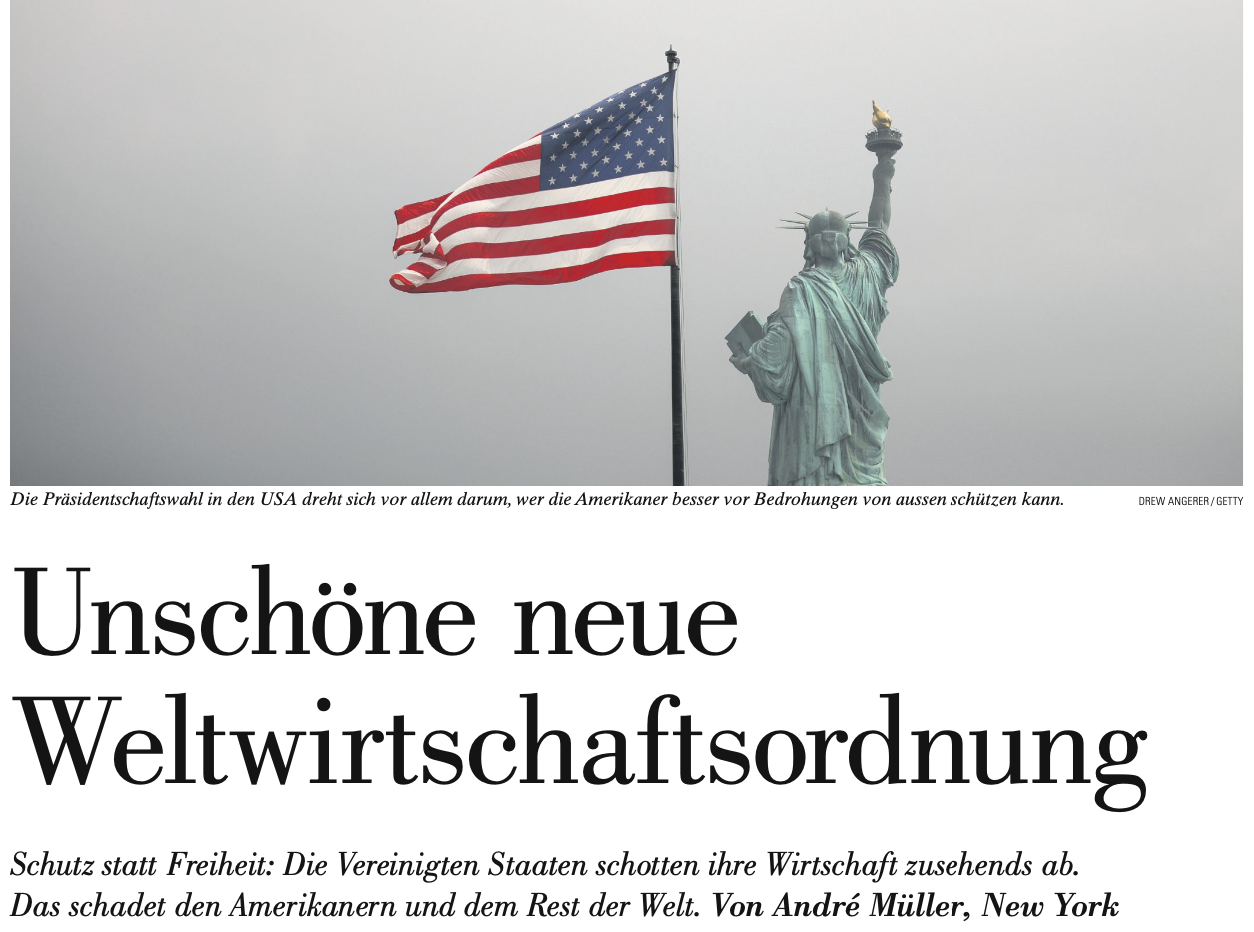
\includegraphics[width=.8\linewidth]{Geografie/LOFS/NZZ-Protektionismus-Headline}
\caption{Titel eines NZZ-Artikels vom 10. Oktober 2024}
\label{fig:nzz-protektionismus-headline}
\end{figure}

Das Wort \enquote{Protektionismus} stammt vom lateinischen \textit{protectio} = Schutz und bedeutet im ursprünglichen Sinn, dass der inländische Handel vom internationalen Wettbewerb gewissermassen abgeschirmt oder \enquote{geschützt} wird. Häufig wird dies erzielt, indem Hindernisse für den internationalen Handel errichtet werden, beispielsweise durch Einfuhrzölle, also Gebühren auf den Import  gewisser ausländischer Waren. Im Gegensatz dazu steht das Konzept des \textbf{Freihandels}, bei welchem, wie es der Name bereits sagt, internationale Handelsflüsse \textit{frei} und ohne Hindernisse stattfinden können. Bei Freihandelsabkommen geht es häufig nicht nur um den Abbau von Einfuhrzöllen, sondern auch um die gegenseitige Anerkennung von Standards und Normen. Dies senkt Kosten, da doppelte Zulassungsverfahren oder Anerkennungsprozeduren zeitaufwendig und teuer sein können \cite[22]{alma99117154311805511}.



\begin{myexercise}[Brainstorming-Aufgabe]
Notieren Sie Vor- und Nachteile der \textbf{Globalisierung} hinsichtlich der Dimensionen \textit{Umwelt}, \textit{Soziales} und \textit{Gesellschaft}
\begin{table}[H]
\centering
\begin{tabular}{c|p{.25\textwidth}|p{.25\textwidth}|p{.25\textwidth}}
& Umwelt & Gesellschaft & Wirtschaft \\\midrule\midrule
Vorteile & & & \\[50pt]\midrule
Nachteile & & & \\[50pt]
\end{tabular}
\end{table}
\begin{myanswer}
Mögliche Antworten (nicht-abschliessend):
\begin{table}[H]
\centering
\small
\begin{tabular}{c|p{.25\textwidth}|p{.25\textwidth}|p{.25\textwidth}}
& Umwelt & Gesellschaft & Wirtschaft \\\midrule\midrule
Vorteile 
& Internationale Zusammenarbeit beim Umweltschutz, Verbreitung umweltfreundlicher Technologien 
& Kultureller Austausch, bessere globale Vernetzung, Zugang zu Bildung und Informationen 
& Grössere Märkte, Spezialisierung, sinkende Produktionskosten, mehr Arbeitsplätze in Schwellenländern \\[50pt]\midrule
Nachteile 
& Umweltverschmutzung durch Transport und Produktion, Ressourcenübernutzung 
& Ungleichheit, Verlust lokaler Kulturen, prekäre Arbeitsbedingungen 
& Abhängigkeit von globalen Märkten, Verlagerung von Arbeitsplätzen, Machtkonzentration bei Grosskonzernen \\[50pt]
\end{tabular}
\end{table}
\end{myanswer}
\end{myexercise}

\begin{myexercise}
Notieren Sie sich während dem Schauen des \href{https://www.youtube.com/watch?v=ksPBr_JL_Oc}{Youtube-Videos}, was mit folgenden Begriffen gemeint ist:

\begin{itemize}
\item Protektionismus
\item Import-Zölle
\item Wettbewerb
\item Protektionsspirale
\item Weltwirtschaftskrise
\end{itemize}

\notiz{8}

\begin{myanswer}
\begin{itemize}
    \item \textbf{Protektionismus}: Wirtschaftspolitische Massnahmen, die darauf abzielen, die heimische Wirtschaft vor ausländischer Konkurrenz zu schützen, z. B. durch Zölle oder Subventionen.
    
    \item \textbf{Import-Zölle}: Abgaben auf Waren, die aus dem Ausland eingeführt werden, um ausländische Produkte teurer zu machen und den Kauf inländischer Produkte zu fördern.
    
    \item \textbf{Wettbewerb}: Der internationale Konkurrenzkampf zwischen Unternehmen, der durch Protektionismus eingeschränkt wird, was zu weniger Innovation und höheren Preisen führen kann.
    
    \item \textbf{Protektionsspirale}: Eine wirtschaftliche Entwicklung, bei der Länder als Reaktion auf protektionistische Massnahmen anderer Staaten selbst Handelsschranken errichten, was den Welthandel zunehmend einschränkt.
    
    \item \textbf{Weltwirtschaftskrise}: Ein extremes Szenario, das eintreten kann, wenn zu viele Länder protektionistische Massnahmen ergreifen, was den internationalen Handel stark reduziert und wirtschaftliche Instabilität verursacht.
\end{itemize}
\end{myanswer}
\end{myexercise}

\begin{myexercise}
Fassen Sie die Hauptargumente aus dem folgenden NZZ-Artikel zusammen, welche für oder gegen Protektionismus sprechen.
\begin{figure}[H]
\centering
\colorbox{white}{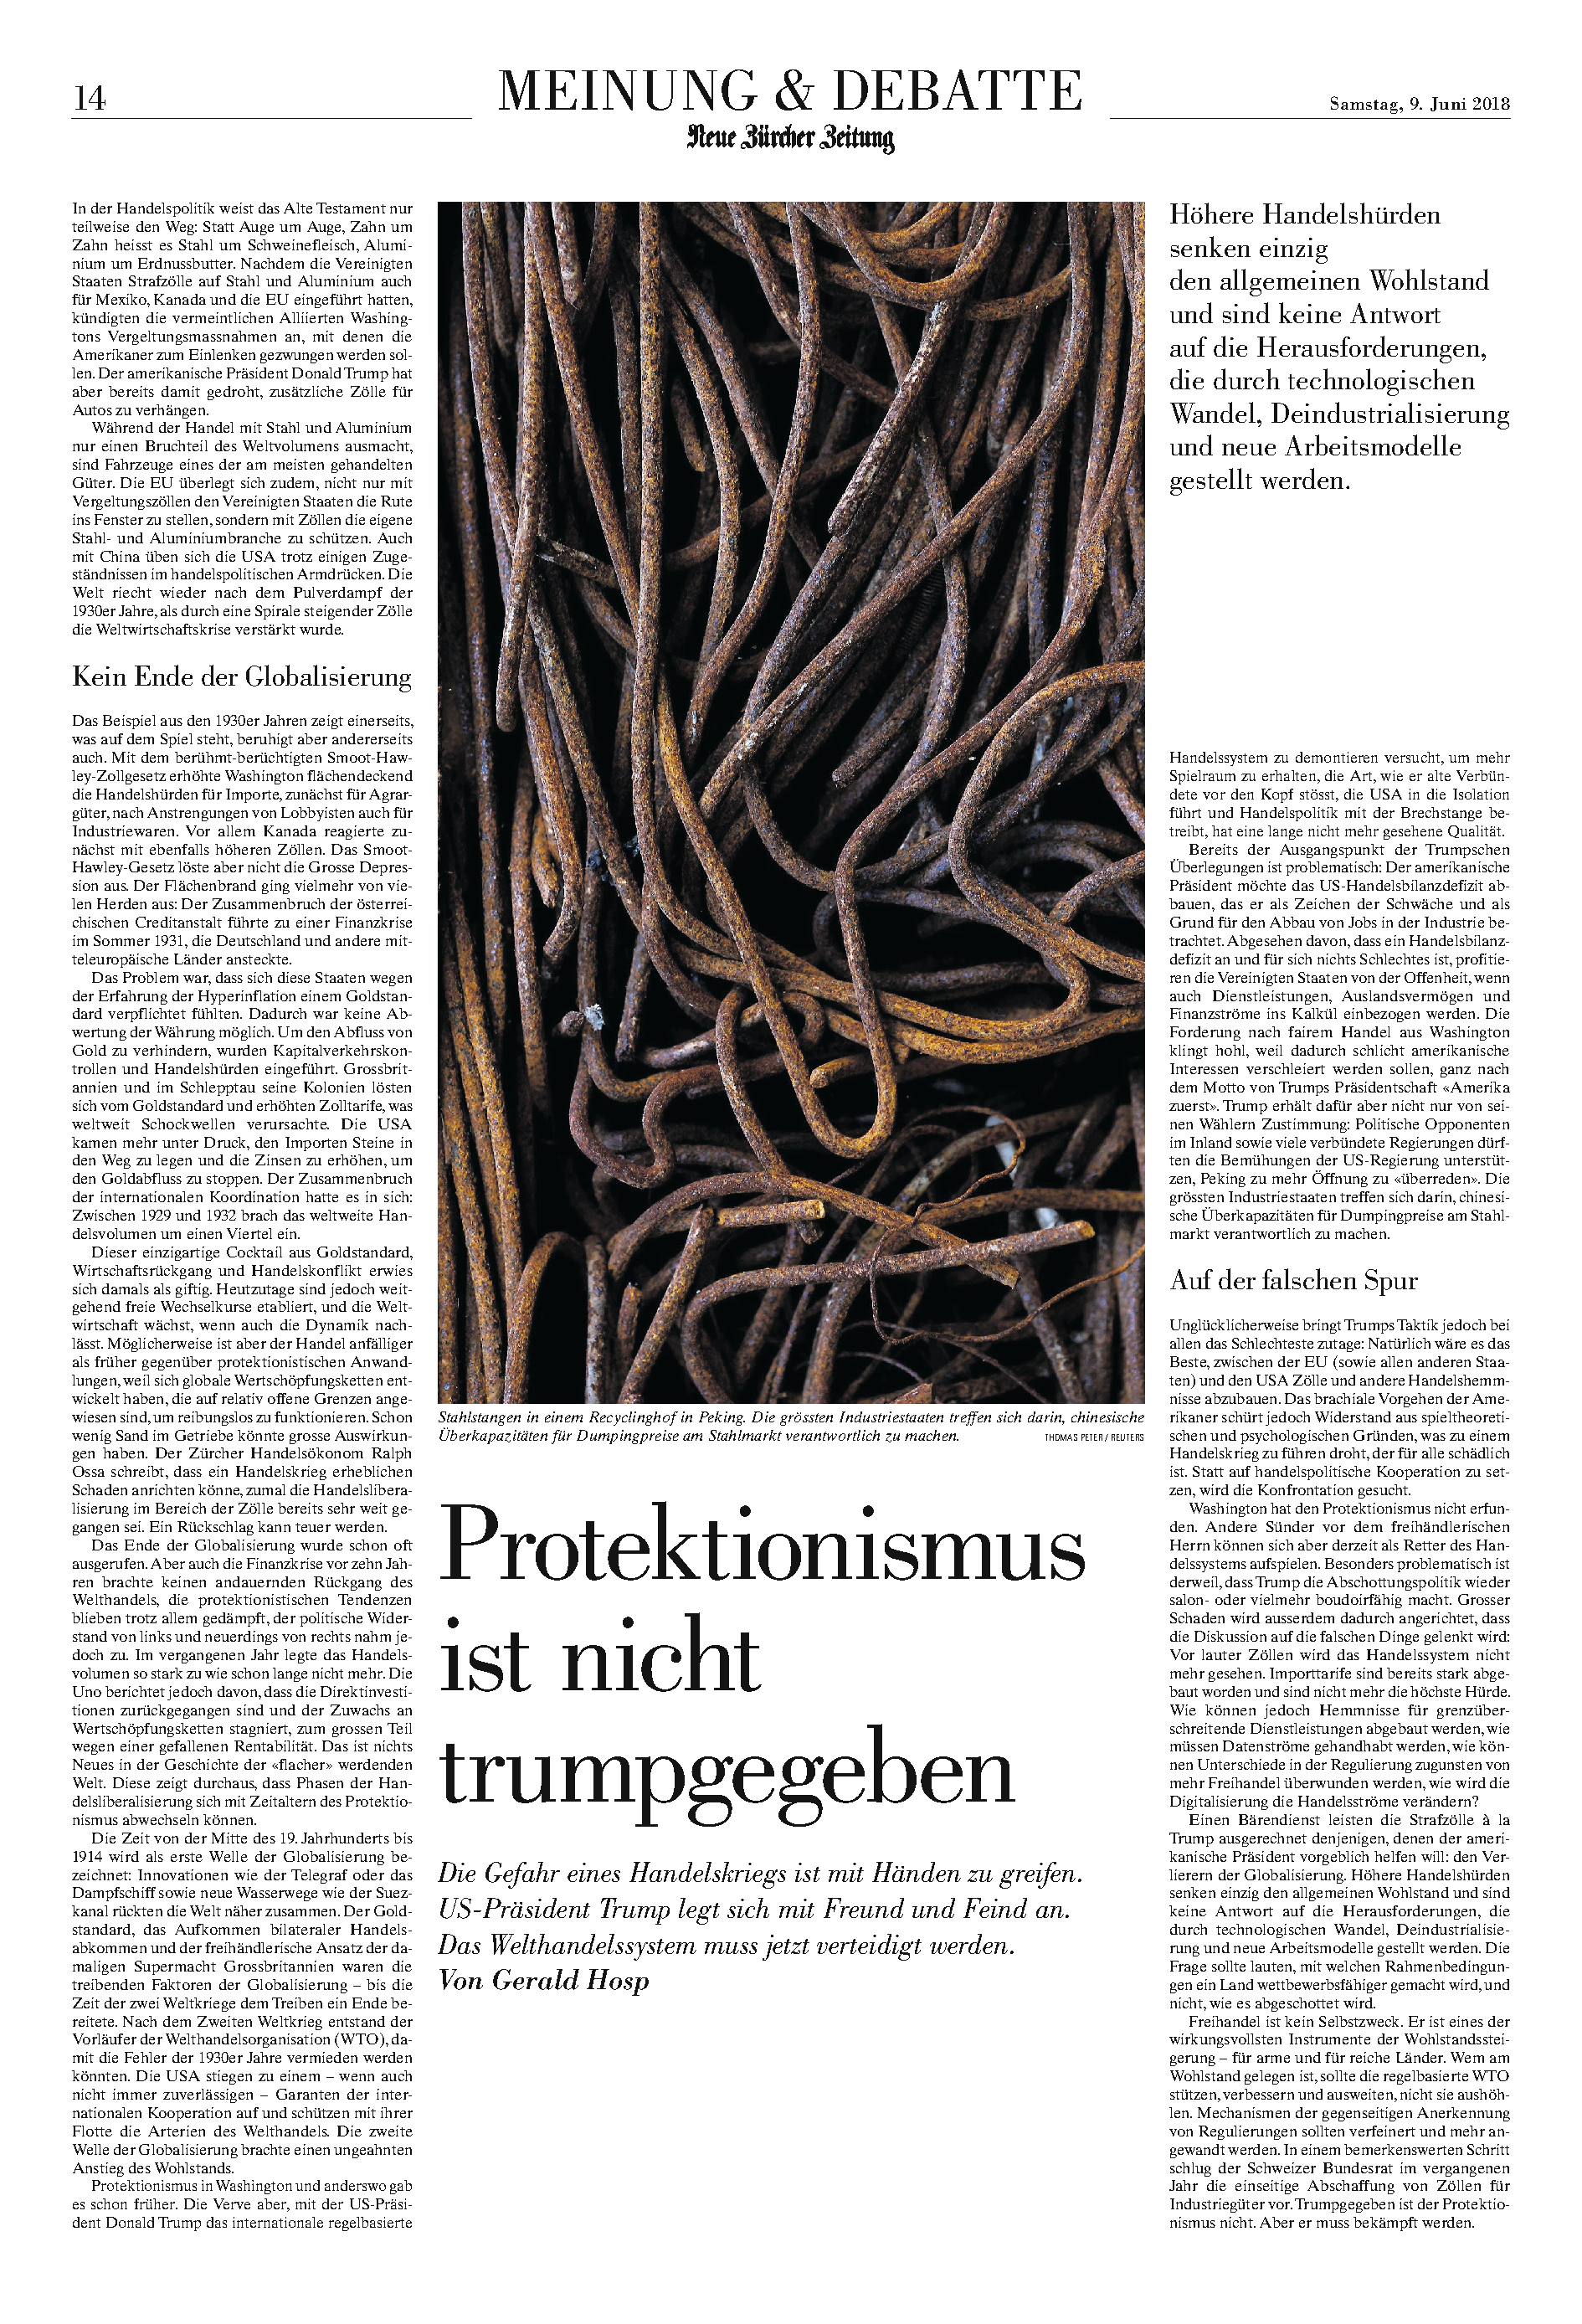
\includegraphics[width=.8\linewidth]{Geografie/LOFS/Seite_14_NZZ_-_Neue_Zürcher_Zeitung_2018-06-09}}
%\caption{NZZ-Artikel über Protektionismus, 09.06.2018}
%\label{fig:seite14nzz-neuezurcherzeitung2018-06-09}
\end{figure}
\begin{myanswer}
Mögliche Antworten:
\begin{table}[H]
    \centering
    \renewcommand{\arraystretch}{1.3}
    \begin{tabular}{p{6cm}|p{6cm}}
        \textbf{Pro Protektionismus} & \textbf{Contra Protektionismus} \\
        \midrule\midrule
        \textbf{Schutz vor Dumping-Preisen}, insbesondere durch chinesische Überkapazitäten & Höhere Handelshürden senken den \textbf{allgemeinen Wohlstand} \\
        \midrule
        \textbf{Unterstützung bestimmter Industrien}, z. B. Stahl- und Aluminiumbranche & Gefahr eines \textbf{Handelskriegs und wirtschaftlicher Instabilität} \\
        \midrule
        Förderung nationaler \textbf{wirtschaftlicher Unabhängigkeit} & \textbf{Rückgang des globalen Handelsvolumens} (historisches Beispiel: 1930er Jahre) \\
        \midrule
        Wirtschaftlicher Druck als \textbf{Verhandlungsstrategie} (z. B. USA gegen China) & Handelskrieg kann die \textbf{Weltwirtschaftskrise verstärken} (1930er-Parallele) \\
        \midrule
        & Protektionismus ist keine Antwort auf \textbf{technologische Veränderungen} oder Deindustrialisierung (verhindert Änderungen nicht) \\
        \midrule
        & \textbf{Verzerrung des globalen Wettbewerbs} und \textbf{Schwächung globaler Wertschöpfungsketten} \\
        \midrule
        & Freihandel ist ein wichtiges Instrument der \textbf{Wohlstandssteigerung} \\
        \midrule
        & Handelsliberalisierung hat \textbf{historisch positive wirtschaftliche Entwicklungen} ermöglicht \\
    \end{tabular}
    \caption{Argumente für und gegen Protektionismus (basierend auf dem NZZ-Artikel)}
    \label{tab:protektionismus}
\end{table}
\end{myanswer}
\end{myexercise}

\begin{myexercise}
Notieren Sie sich beim Anhören des \href{https://www.srf.ch/news/wirtschaft/wirtschaft-textilbranche-will-sich-selbst-helfen-und-die-zoelle-abschaffen}{SRF-Audios}, weshalb die Schweizer Textilbranche für einen Abbau von Zöllen ist. 

\notiz{6}

\begin{myanswer}
\begin{itemize}
\item Schweizer Textilfirmen müssen ebenfalls Zölle für Rohstoff-Importe (Textil-Fasern, etc.) zahlen.
\item Textilien werden nicht mehr von A-Z hergestellt, man ist also international abhängig und Teil eines komplexen internationalen Geflechts..
\end{itemize}
\end{myanswer}
\end{myexercise}

\begin{mychallenge}[NZZ-Artikel zu Protektionismus in den USA]
\begin{figure}[H]
\centering
\colorbox{white}{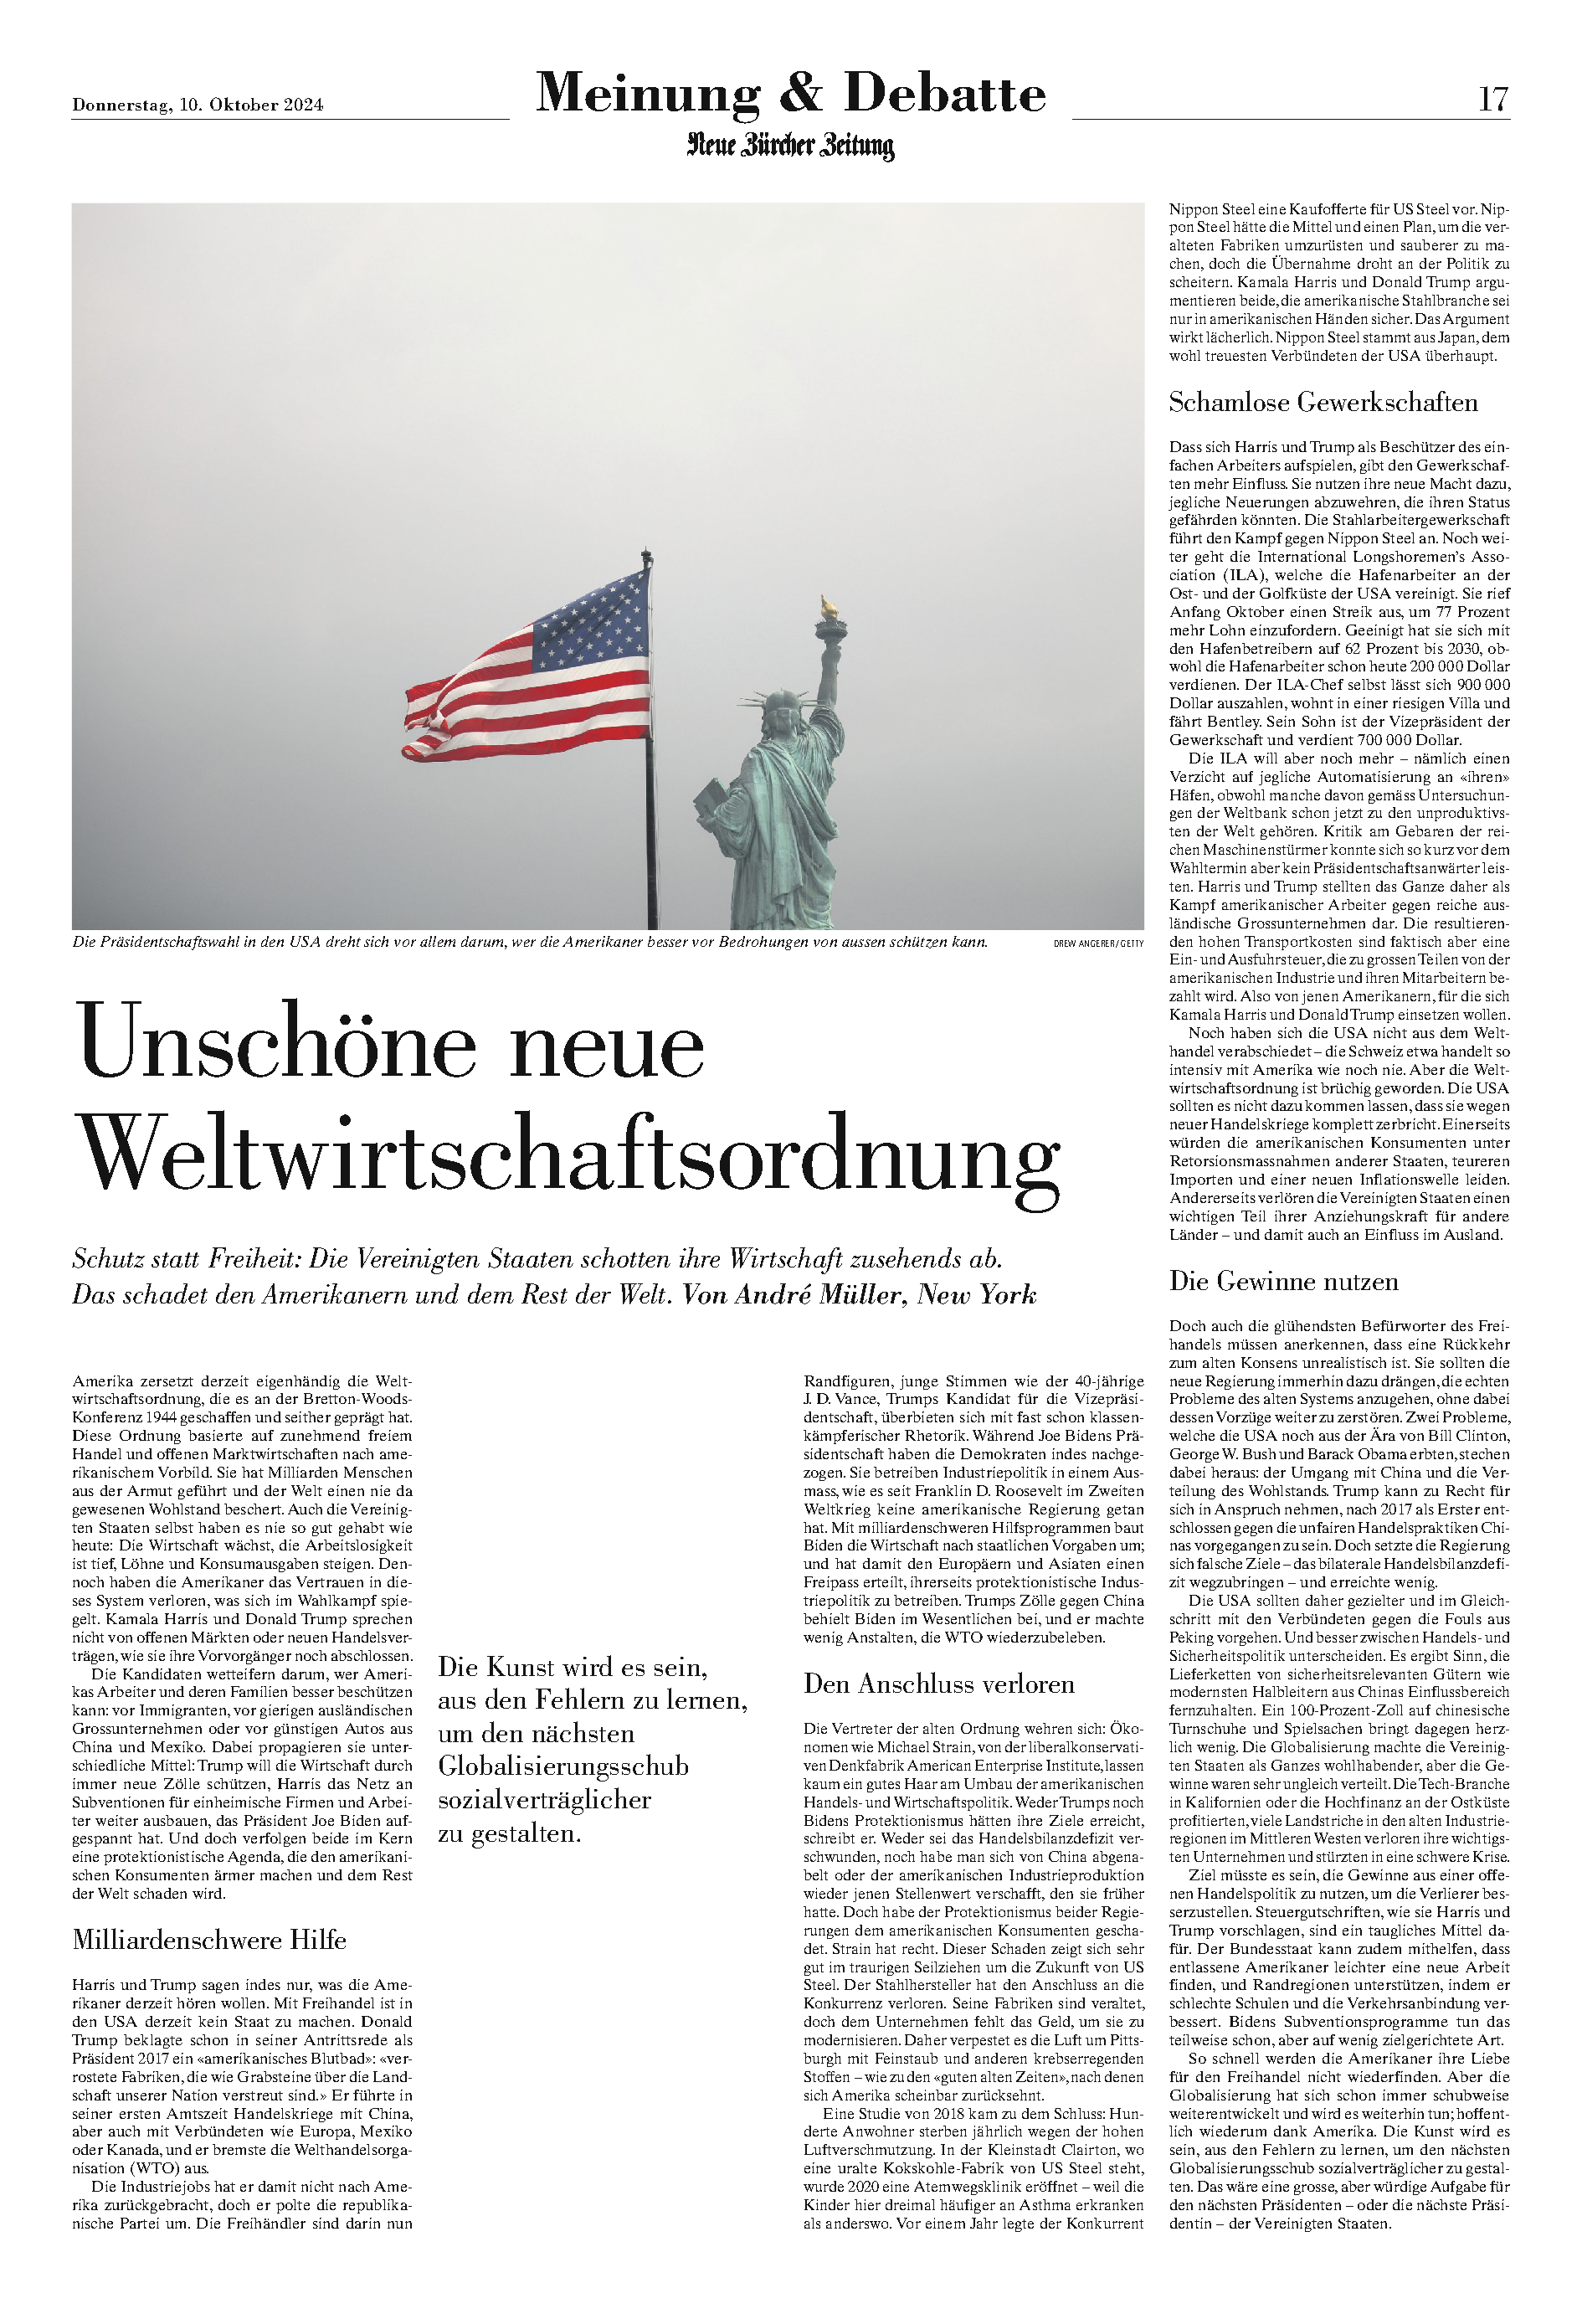
\includegraphics[width=.9\linewidth]{Geografie/LOFS/Seite_17_NZZ_-_Neue_Zürcher_Zeitung_2024-10-10}}
\end{figure}
\end{mychallenge}

\clearpage
\chapter{Grüne Globalisierung -- Nachhaltige Zukunftsperspektiven?}

Die Verfügbarkeit grösserer Mengen an Energie (vor allem Erdöl) war die Voraussetzung für die Entstehung des globalen Welthandels \cite[266]{hep}. Gerade der hohe Energie- und Ressourcen-Verbrauch globaler Wertschöpfungsketten haben vielerorts Kritik hervorgerufen. In dieser Doppellektion widmen wir uns einigen nicht-protektionistischen Ansätzen, um globale Wertschöpfungsketten nachhaltiger zu gestalten. Dabei liegt der Hauptfokus darin, ein beschränkte Ressourcen gezielter einzusetzen \cite[486]{westermann}.

\begin{myexercise}[Gruppen-Puzzle zu Nachhaltigkeits-Prinzipien]
Lesen Sie zunächst \textit{individuell} einen der folgenden Texten zu den Konzepten \textit{Effizienz}, \textit{Konsistenz} und \textit{Suffizienz}.

Fassen Sie ihr Konzept danach anhand von \textbf{drei Schlüsselbegriffen} zusammen und suchen Sie sich \textbf{drei zum Konzept passende Bilder} von der Vorlage aus (s. \cref{fig:beispielbildernachhaltigkeit}).

Setzten Sie sich nach dem Lesen der Konzepte in 3er-Gruppen zusammen und erklären Sie sich gegenseitig die Nachhaltigkeits-Konzepte anhand Ihrer 3 Schlüsselbegriffe und Ihrer 3 Bilder.

\begin{textBox}[title = Suffizienz -- anders konsumieren für ein gutes Leben für alle \cite{suffizienz}]

Suffizienz hat seine Wurzeln im lateinischen „sufficere“, was soviel wie „ausreichen“ bedeutet. Suffizienz stellt die Frage nach dem rechten Mass. Es geht darum, zu überlegen: Wie viel brauche ich wirklich? Was ist für ein gutes Leben wichtig? Das Ziel ist, weniger Rohstoffe und Energie zu verbrauchen, indem wir weniger kaufen und nutzen – vor allem Dinge, die unsere Lebensqualität kaum verbessern.

Wichtige Fragen dabei sind: Welche Bedürfnisse müssen erfüllt sein, um ein gutes Leben zu führen? Es geht nicht nur um materielle Dinge. Oft werden durch Werbung oder neue Technologien künstlich neue Wünsche geweckt, die wir gar nicht brauchen. 

Suffizienz kann helfen, sich vom Überfluss zu befreien. So können Menschen entdecken, wie wichtig soziale Kontakte, emotionale Ausgeglichenheit und kulturelle Erlebnisse sind.

Ein Leben, in dem Menschen genug, aber nicht zu viel haben, kann Beziehungen stärken. Es kann Menschen glücklicher und unabhängiger von materiellen Dingen machen.

Suffizienz setzt also nicht auf der Produktionsseite an, sondern auf bei Konsummustern. Daher geraten auch kulturelle und soziale Aspekte unserer Lebensweise in den Blick.
\end{textBox}

\begin{textBox}[title = Konsistenz -- anders herstellen und
nutzen \cite{konsistenz}]

Konsistenz bedeutet, dass Produktion und Konsum wie ein Kreislauf funktionieren – ohne Müll. Alles wird wiederverwertet, wie in der Natur. 

Ein Kirschbaum produziert viele Blüten und Früchte. Wenn diese auf den Boden fallen und verrotten, schaden sie der Umwelt nicht. Stattdessen werden sie zu Dünger und Nahrung
für Kleinstlebewesen – alles bleibt Teil eines Kreislaufs.

Konsistenz will also Ressourcen immer wieder verwenden. Das nennt man auch \enquote{cradle to cradle} (\enquote{von der Wiege zur Wiege}): Produkte werden so gemacht, dass sie nie zu Abfall werden.

Das funktioniert auf zwei Arten:

\begin{enumerate}
\item \textbf{Biologisch abbaubare Materialien}: Diese können komplett kompostiert werden.

\item \textbf{Technische Materialien}: Diese bleiben im Kreislauf und werden immer wiederverwendet. Zum Beispiel könnten Computergehäuse ständig genutzt werden, indem man nur die Elektronik austauscht. So entstehen keine Abfälle, sondern neue Produkte oder sogar bessere („Upcycling“).
\end{enumerate}
Konsistenz als Nachhaltigkeitsstrategie setzt auf der Produktionsseite an.
\end{textBox}

\begin{textBox}[title = Effizienz -- besser produzieren mit weniger Ressourcenverbrauch und CO$_2$-Ausstoss \cite{effizienz}]


Das Verhältnis zwischen Aufwand/Input und Nutzen/Output verbessert sich fortwährend. Das bedeutet: Die hergestellte Menge eines Produkts bleibt gleich oder steigt, während zugleich die Menge der dafür eingesetzten Ressourcen (Rohstoffe, Energie, Zeit, Arbeitskraft) sinkt oder gleich bleibt. Die Idee ist, mit möglichst wenig, möglichst viel zu erreichen.

Ökoeffizienz weist nun vor allem auf die eingesetzten natürlichen Ressourcen sowie den Müll und die Emissionen hin, die im Produktionsprozess entstehen. Ökoeffizienz schliesst ebenfalls den Betrieb eines Produkts selbst ein – also etwa Strom- oder Wasserverbrauch. Die Effizienzstrategie konzentriert sich auf die Produktion und setzt auf technologische Fortschritte.

Da der geringere Verbrauch an Material, Energie, Arbeitskraft und Zeit etc. für Unternehmen auch mit grossen finanziellen Einsparpotentialen verbunden ist, wird in vielen Branchen kontinuierlich auf Effizienzsteigerung gesetzt. Ökoeffizienz hat also nicht nur ökologische, sondern auch betriebswirtschaftliche Vorteile im ökonomischen Wettbewerb.
\end{textBox}

\begin{figure}[H]
\centering
\colorbox{white}{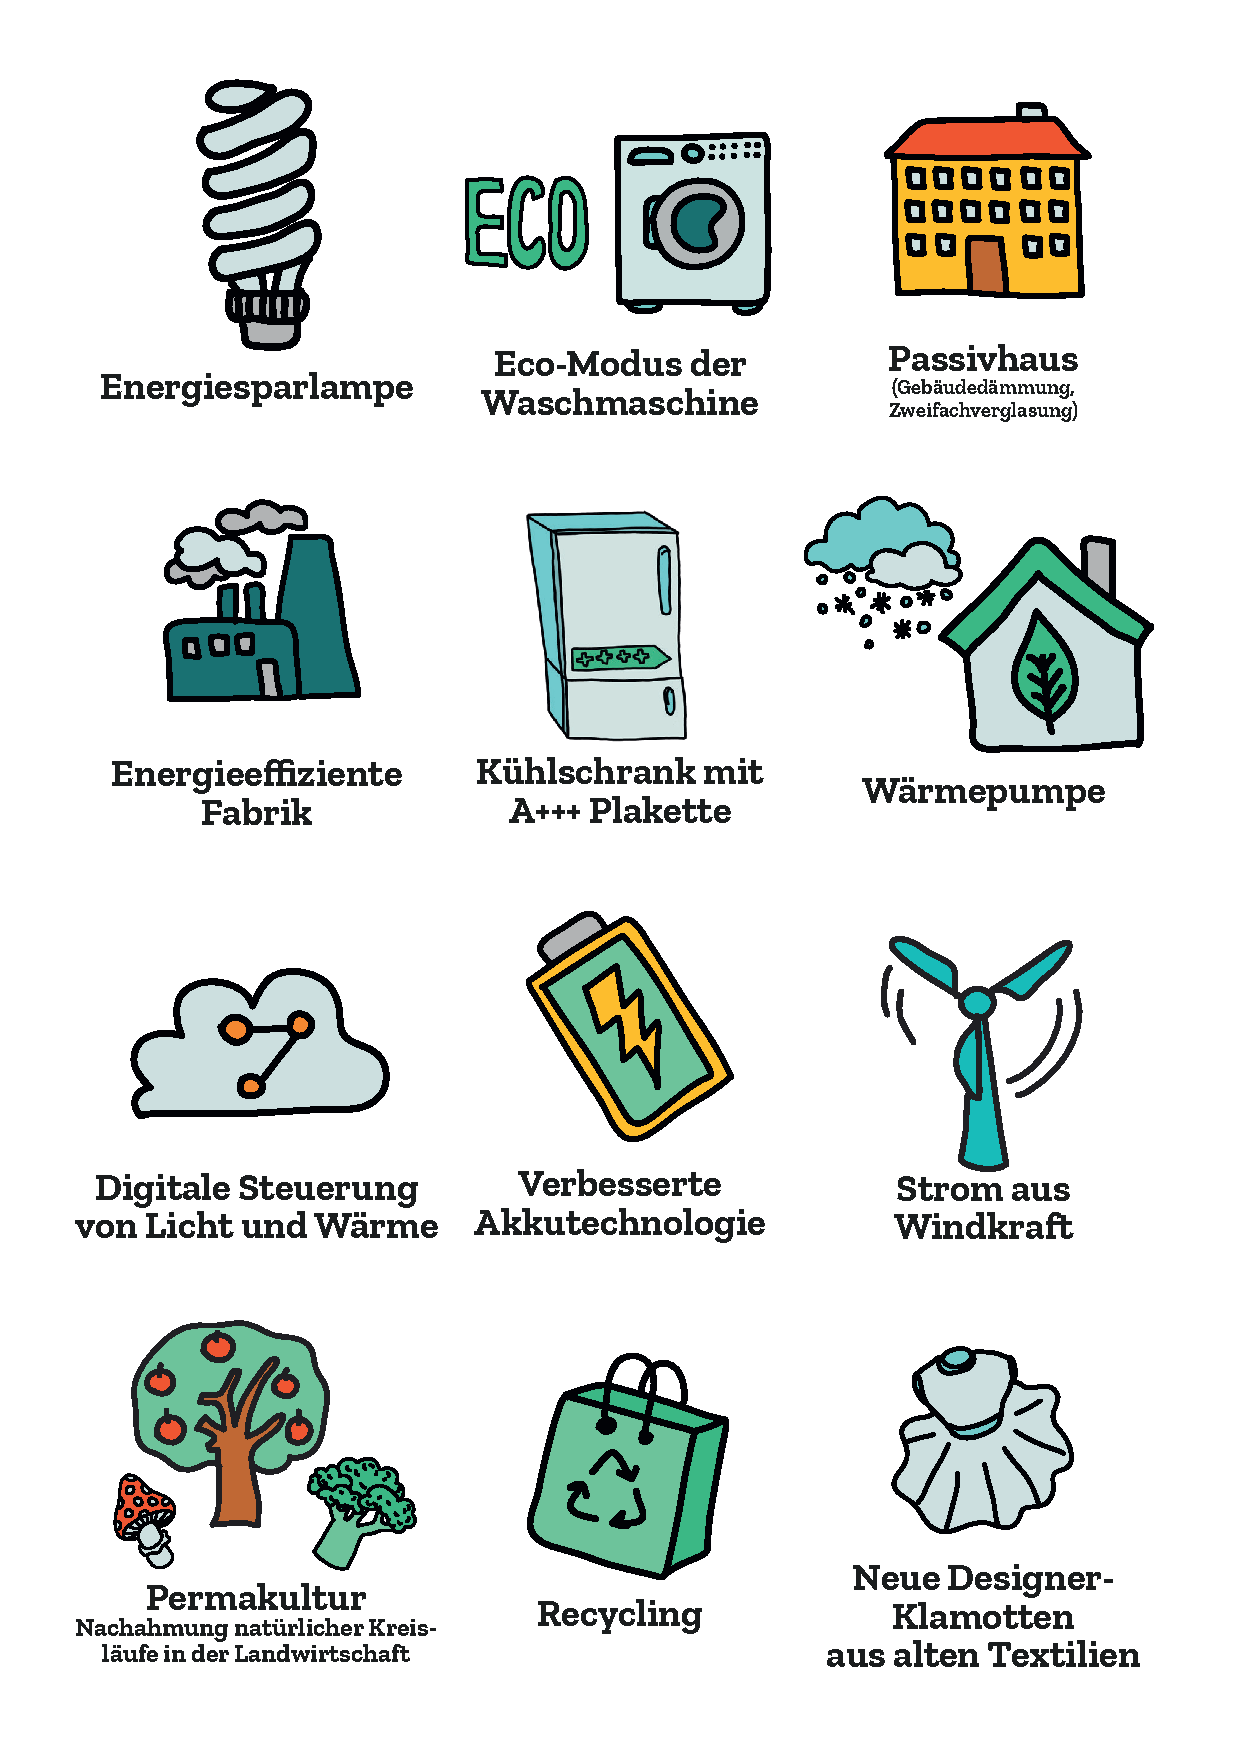
\includegraphics[width=0.45\linewidth, page=1]{Geografie/LOFS/Beispielbilder_Nachhaltigkeit}
\includegraphics[width=0.45\linewidth, page=2]{Geografie/LOFS/Beispielbilder_Nachhaltigkeit}}
\caption{Bilder zu Nachhaltigkeits-Konzepten Suffizienz, Konsistenz und Effizienz \cite{strategienNachhaltigkeit}}
\label{fig:beispielbildernachhaltigkeit}
\end{figure}



\begin{myanswer}
3 Schlüsselbegriffe (mögliche Lösung)
\begin{itemize}
    \item \textbf{Suffizienz}
    \begin{itemize}
        \item \textbf{ausreichen} (Wurzeln im lateinischen „sufficere“)
        \item \textbf{Lebensqualität} (nicht nur materielle Dinge sind wichtig)
        \item \textbf{Konsum} (Veränderung der Konsummuster)
    \end{itemize}

    \item \textbf{Konsistenz}
    \begin{itemize}
        \item \textbf{Kreislauf} (Produktion und Konsum ohne Müll)
        \item \textbf{wiederverwerten} (alles bleibt Teil des Systems)
        \item \textbf{biologisch abbaubar} (Materialien sollen nachhaltig nutzbar sein)
    \end{itemize}

    \item \textbf{Effizienz}
    \begin{itemize}
        \item \textbf{Input-Output-Verhältnis} (Verhältnis zwischen Aufwand und Nutzen verbessern)
        \item \textbf{Ökoeffizienz} (Fokus auf Umweltaspekte)
        \item \textbf{Ressourcenverbrauch} (Reduktion von Rohstoffen, Energie, Emissionen)
    \end{itemize}
\end{itemize}
Bei den Bilder-Auswahlen sind viele Lösungen möglich.
\end{myanswer}

\end{myexercise}

\begin{myexercise}[Gruppen-Puzzle zu Nachhaltigkeits-Konzepten]

Dieser Auftrag besteht aus mehreren Teilen:

\begin{enumerate}
\item Schauen Sie sich zunächst \textit{individuell} eines der folgenden drei Videos (Quelle: \textcite{globalGreenEconomy}) an und notieren Sie sich in 3 Schlüsselbegriffen, worum es geht. Notieren Sie sich ebenfalls, welches der Nachhaltigkeits-Konzepte Effizienz, Suffizienz und Konsistenz Sie im jeweiligen Konzept wiedererkennen können?
\begin{table}[H]
\centering
\begin{tabular}{c|c}
\textbf{Konzept} & \textbf{Link (anklickbar)} \\
\midrule\midrule
Kreislaufwirtschaft / Circular Economy & \qrcode[height=1.5cm]{https://www.youtube.com/watch?time_continue=2&v=0lDgaptvbD0&feature=emb_logo} \\\midrule
Gemeinwohlökonomie & \qrcode[height=1.5cm]{https://www.youtube.com/watch?v=cVFvyd7SmxU&feature=emb_logo} \\\midrule
Degrowth & \qrcode[height=1.5cm]{https://vimeo.com/121263974} \\\midrule
Cradle-to-Cradle & \qrcode[height=1.5cm]{https://www.youtube.com/watch?v=g1tIGLy3PHw&feature=emb_logo} 
\end{tabular}
\end{table}
\item Setzen Sie sich danach in ihre ursprünglichen Gruppen (nach globalem Produkt: Schokolade, Smartphone etc.) zusammen und erklären Sie sich die Konzepte gegenseitig, indem Sie folgende Tabelle vervollständigen. Setzen Sie bei den letzten drei Spalten lediglich Häkchen oder Kreuze.

\begin{table}[H]
    \centering
    \small
    \begin{tabular}{ c | p{3.5cm} | p{2cm} | p{2cm} | p{2cm} }
        \textbf{Konzept} & \textbf{Schlüsselbegriffe} & \textbf{Effizienz} & \textbf{Suffizienz} & \textbf{Konsistenz} \\
        \midrule
        Kreislaufwirtschaft & &  &  &  \\[50pt]\midrule
        GWÖ &  &  &  &  \\[50pt]\midrule
        Degrowth &  &  &  &  \\[50pt]\midrule
        Cradle-to-Cradle & &  &  & \\[50pt]
    \end{tabular}
    \caption{Schlüsselbegriffe und Nachhaltigkeitsstrategien der Konzepte}
\end{table}

\item Bestimmen Sie \textit{nach} dem Austausch in Ihren Produkte-Gruppen \textit{ein} Konzept, welches besonders geeignet wäre, um die Nachhaltigkeits Ihres globalen Produktes zu verbessern.
\end{enumerate}

\begin{myanswer}
\begin{table}[H]
    \centering
    \small
    \begin{tabular}{ c | p{3.5cm} | c | c | c }
        \textbf{Konzept} & \textbf{Schlüsselbegriffe} & \textbf{Effizienz} & \textbf{Suffizienz} & \textbf{Konsistenz} \\
        \midrule
        Kreislaufwirtschaft & Ressourcenwiederverwendung, Kaskadennutzung, Recycling-Technologien & \checkmark &  & \checkmark \\\midrule
        GWÖ & Nachhaltige Unternehmen, soziale Gerechtigkeit, ethische Anreize &  & \checkmark & \checkmark \\\midrule
        Degrowth & Postwachstum, Wachstumszwänge hinterfragen, alternative Gesellschaftsmodelle &  & \checkmark & \checkmark \\\midrule
        Cradle-to-Cradle & Biologische und technische Kreisläufe, abfallfreies Design, positive Ökobilanz & \checkmark &  & \checkmark \\
    \end{tabular}
    \caption{Schlüsselbegriffe und Nachhaltigkeitsstrategien der Konzepte}
    \label{tab:nachhaltigkeitskonzepte}
\end{table}


\end{myanswer}
\end{myexercise}
